\documentclass{report}
\usepackage[utf8]{inputenc}

\usepackage[rgb]{xcolor}

\usepackage{geometry}
\usepackage{tikz}

% Saves PDFs of each Tikz Feynman Diagram.
% Logs and output files (next to Recompile) -> Other logs and files -> output-fileX.pdf
\usetikzlibrary{external}
\tikzexternalize[prefix=tikz/]

\usepackage[compat=1.1.0]{tikz-feynman}
\usepackage{subcaption}

% HH sub-group hex colour codes:
\definecolor{hh_pink}{HTML}{F2385A}
\definecolor{hh_blue}{HTML}{343844}
\definecolor{hh_med_turq}{HTML}{36B1BF}
\definecolor{hh_lgt_turq}{HTML}{4AD9D9}
\definecolor{hh_whte}{HTML}{E9F1DF}
\definecolor{hh_yllw}{HTML}{FDC536}
%\definecolor{hh_gren}{HTML}{125125}
\definecolor{hh_gren}{HTML}{00CC00}


\begin{document}

\newgeometry{vmargin={30mm}, hmargin={12mm,17mm}}

\begin{figure}
\centering
    \begin{subfigure}[t]{0.49\textwidth}
        \centering
        
        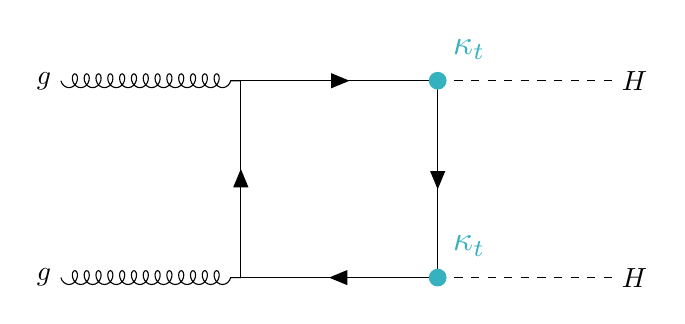
\begin{tikzpicture}
            \begin{feynman}
                
                \vertex(g1) at (-3.75, -1.25) {\(g\)};
                \vertex(g2) at (-3.75, 1.25) {\(g\)};
                
                \vertex (t1) at (-1.25, -1.25);
                \vertex (t2) at (-1.25, 1.25);
                \vertex (t3) at (1.25, 1.25);
                \vertex (t4) at (1.25, -1.25);
            
                \vertex (h1) at (3.75, -1.25) {\(H\)};
                \vertex (h2) at (3.75, 1.25) {\(H\)};

                \diagram*{
                    (g1) -- [gluon] (t1),
                    (g2) -- [gluon] (t2),
                    (t1) -- [fermion] (t2) -- [fermion] (t3) -- [fermion] (t4) -- [fermion] (t1),
                    (t3) -- [scalar] (h2),
                    (t4) -- [scalar] (h1)
                    
                };
                
            \end{feynman}

        \filldraw [hh_med_turq] (1.25, 1.25) circle (3pt);
        \node[hh_med_turq, scale=1.25] at (1.65, 1.65) {\(\kappa_{t}\)};
        \filldraw [hh_med_turq] (1.25, -1.25) circle (3pt);
        \node[hh_med_turq, scale=1.25] at (1.65, -0.85) {\(\kappa_{t}\)};

        \end{tikzpicture}
    
    \caption{}
    \end{subfigure}%
    \begin{subfigure}[t]{0.49\textwidth}
        \centering
        
        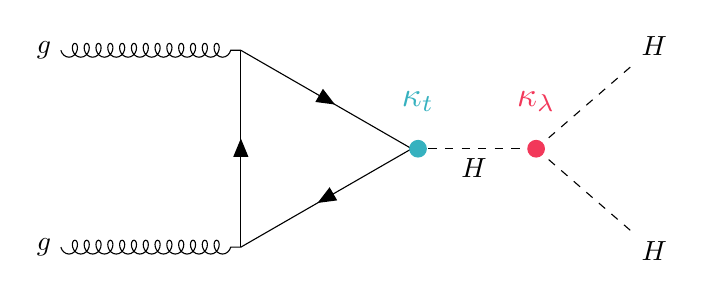
\begin{tikzpicture}
            \begin{feynman}
                
                \vertex(g1) at (-3.75, -1.25) {\(g\)};
                \vertex(g2) at (-3.75, 1.25) {\(g\)};
                
                \vertex (t1) at (-1.25, -1.25);
                \vertex (t2) at (-1.25, 1.25);
                \vertex (t3) at (0.92, 0);
                
                \vertex (h1) at (2.5, 0);
                \vertex (h2) at (4.0, 1.3) {\(H\)};
                \vertex (h3) at (4.0, -1.3) {\(H\)};

                \diagram*{
                    (g1) -- [gluon] (t1),
                    (g2) -- [gluon] (t2),
                    
                    (t1) -- [fermion] (t2) -- [fermion] (t3) -- [fermion] (t1),
                    
                    (t3) -- [scalar, edge label'=\(H\)] (h1) -- [scalar] {(h2), (h3)}
                    
                };
                
            \end{feynman}

        \filldraw [hh_med_turq] (1.0, 0) circle (3pt);
        \node[hh_med_turq, scale=1.25] at (1.0, 0.6) {\(\kappa_{t}\)};
        \filldraw [hh_pink] (2.5, 0) circle (3pt);
        \node[hh_pink, scale=1.25] at (2.5, 0.6) {\(\kappa_{\lambda}\)};
        
        \end{tikzpicture}
    
    \caption{}
    \end{subfigure}%
\caption{The two tree-level Feynman Diagrams for di-Higgs production via Gluon-Gluon Fusion.}
\end{figure}

\begin{figure}
\centering
    \begin{subfigure}[t]{0.33\textwidth}
        \centering
        
        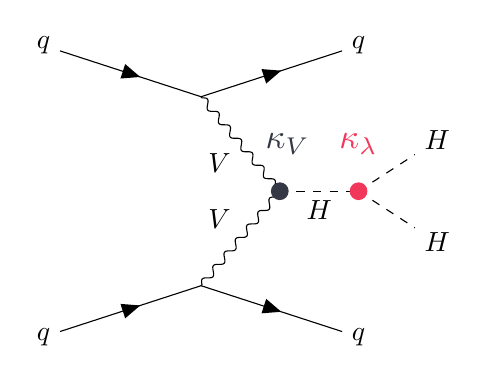
\begin{tikzpicture}
            \begin{feynman}
                \vertex (h1) at (0, 0);
                \vertex (h2) at (1, 0);
                \vertex (h3) at (2, 0.65) {\(H\)};
                \vertex (h4) at (2, -0.65) {\(H\)};
                
                \vertex(V1) at (-1, 1.2);
                \vertex(V2) at (-1, -1.2);
                
                \vertex(q1) at (-3, 1.85) {\(q\)};
                \vertex(q3) at (1, 1.85) {\(q\)};
                \vertex(q2) at (-3, -1.85) {\(q\)};
                \vertex(q4) at (1, -1.85) {\(q\)};

                \diagram*{
                    (h1) -- [scalar, edge label'=\(H\)] (h2) -- [scalar] {(h3), (h4)},
                    (q1) -- [fermion] (V1) -- [fermion] (q3), 
                    (q2) -- [fermion] (V2) -- [fermion] (q4),
                    (V1) -- [boson, edge label'=\(V\)] (h1),
                    (V2) -- [boson, edge label=\(V\)] (h1)
                };
                
            \end{feynman}
        
            \filldraw [hh_pink] (1, 0) circle (3pt);
            \node[hh_pink, scale=1.25] at (1, 0.6) {\(\kappa_{\lambda}\)};
            \filldraw [hh_blue] (0, 0) circle (3pt);
            \node[hh_blue, scale=1.25] at (0.1, 0.6) {\(\kappa_{V}\)};
        
        \end{tikzpicture}
    
    \caption{}
    \end{subfigure}%
    \begin{subfigure}[t]{0.33\textwidth}
        \centering
        
        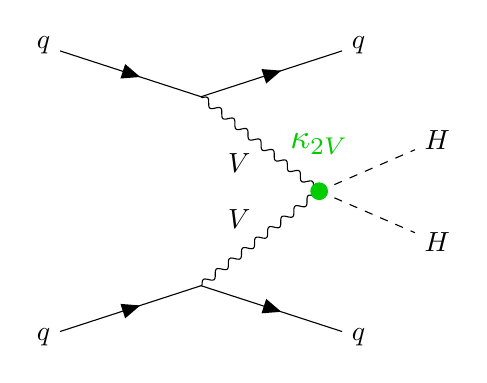
\begin{tikzpicture}
            \begin{feynman}
                \vertex (h2) at (0.5, 0);
                \vertex (h3) at (2, 0.65) {\(H\)};
                \vertex (h4) at (2, -0.65) {\(H\)};
                
                \vertex(V1) at (-1, 1.2);
                \vertex(V2) at (-1, -1.2);
                
                \vertex(q1) at (-3, 1.85) {\(q\)};
                \vertex(q3) at (1, 1.85) {\(q\)};
                \vertex(q2) at (-3, -1.85) {\(q\)};
                \vertex(q4) at (1, -1.85) {\(q\)};

                \diagram*{
                    (h2) -- [scalar] {(h3), (h4)},
                    (q1) -- [fermion] (V1) -- [fermion] (q3), 
                    (q2) -- [fermion] (V2) -- [fermion] (q4),
                    (V1) -- [boson, edge label'=\(V\)] (h2),
                    (V2) -- [boson, edge label=\(V\)] (h2)
                };
                
            \end{feynman}
        
            \filldraw [hh_gren] (0.5, 0) circle (3pt);
            \node[text=hh_gren, scale=1.25] at (0.5, 0.6) {{ \(\kappa_{2V}\) } };
        
        \end{tikzpicture}
    
    \caption{}
    \end{subfigure}%
    \begin{subfigure}[t]{0.33\textwidth}
        \centering
        
        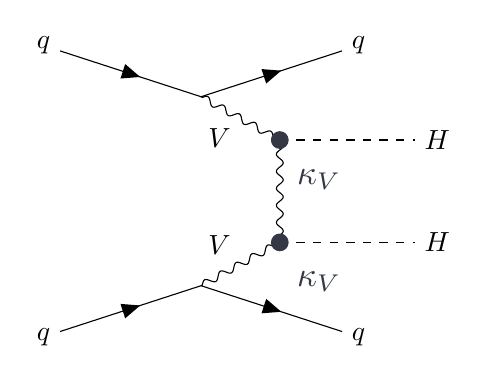
\begin{tikzpicture}
            \begin{feynman}
                \vertex (h1) at (0, 0.65);
                \vertex (h2) at (0, -0.65);
                \vertex (h3) at (2, 0.65) {\(H\)};
                \vertex (h4) at (2, -0.65) {\(H\)};
                
                \vertex(V1) at (-1, 1.2);
                \vertex(V2) at (-1, -1.2);
                
                \vertex(q1) at (-3, 1.85) {\(q\)};
                \vertex(q3) at (1, 1.85) {\(q\)};
                \vertex(q2) at (-3, -1.85) {\(q\)};
                \vertex(q4) at (1, -1.85) {\(q\)};

                \diagram*{
                    (h1) -- [scalar] (h3),
                    (h2) -- [scalar] (h4),
                    (q1) -- [fermion] (V1) -- [fermion] (q3), 
                    (q2) -- [fermion] (V2) -- [fermion] (q4),
                    (V1) -- [boson, edge label'=\(V\)] (h1),
                    (V2) -- [boson, edge label=\(V\)] (h2),
                    (h1) -- [boson] (h2)
                };
                
            \end{feynman}
            
            \filldraw [hh_blue] (0, 0.65) circle (3pt);
            \node[hh_blue, scale=1.25] at (0.5, 0.15) {\(\kappa_{V}\)};
            
            \filldraw [hh_blue] (0, -0.65) circle (3pt);
            \node[hh_blue, scale=1.25] at (0.5, -1.15) {\(\kappa_{V}\)};
        
        \end{tikzpicture}
    
    \caption{}
    \end{subfigure}
\caption{The three tree-level Feynman Diagrams for di-Higgs production via Vector Boson Fusion.}
\end{figure}

\begin{figure}
\centering
    \begin{subfigure}[t]{0.49\textwidth}
        \centering
        
            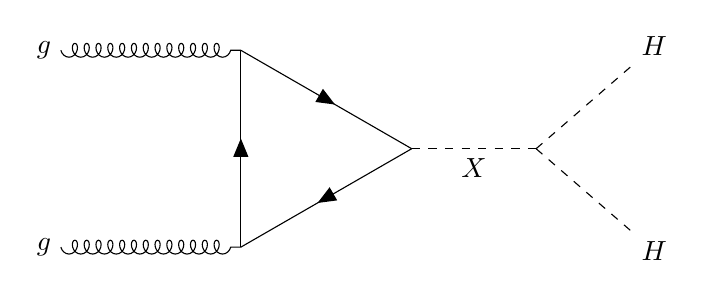
\begin{tikzpicture}
                \begin{feynman}
                    
                    \vertex(g1) at (-3.75, -1.25) {\(g\)};
                    \vertex(g2) at (-3.75, 1.25) {\(g\)};
                    
                    \vertex (t1) at (-1.25, -1.25);
                    \vertex (t2) at (-1.25, 1.25);
                    \vertex (t3) at (0.92, 0);
                    
                    \vertex (h1) at (2.5, 0);
                    \vertex (h2) at (4.0, 1.3) {\(H\)};
                    \vertex (h3) at (4.0, -1.3) {\(H\)};
    
                    \diagram*{
                        (g1) -- [gluon] (t1),
                        (g2) -- [gluon] (t2),
                        
                        (t1) -- [fermion] (t2) -- [fermion] (t3) -- [fermion] (t1),
                        
                        (t3) -- [scalar, edge label'=\(X\)] (h1) -- [scalar] {(h2), (h3)}
                        
                    };
                    
                \end{feynman}
            
            \end{tikzpicture}
    
    \caption{}
    \end{subfigure}%
    \begin{subfigure}[t]{0.49\textwidth}
        \centering
        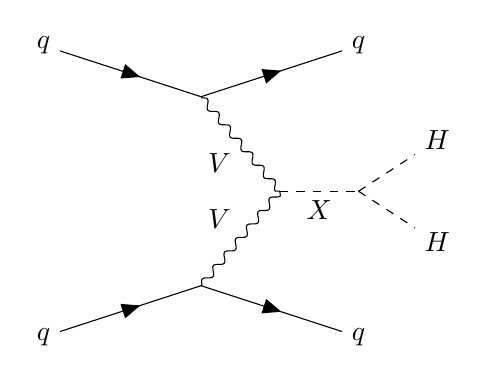
\begin{tikzpicture}
            \begin{feynman}
                \vertex (h1) at (0, 0);
                \vertex (h2) at (1, 0);
                \vertex (h3) at (2, 0.65) {\(H\)};
                \vertex (h4) at (2, -0.65) {\(H\)};
                
                \vertex(V1) at (-1, 1.2);
                \vertex(V2) at (-1, -1.2);
                
                \vertex(q1) at (-3, 1.85) {\(q\)};
                \vertex(q3) at (1, 1.85) {\(q\)};
                \vertex(q2) at (-3, -1.85) {\(q\)};
                \vertex(q4) at (1, -1.85) {\(q\)};
    
                \diagram*{
                    (h1) -- [scalar, edge label'=\(X\)] (h2) -- [scalar] {(h3), (h4)},
                    (q1) -- [fermion] (V1) -- [fermion] (q3), 
                    (q2) -- [fermion] (V2) -- [fermion] (q4),
                    (V1) -- [boson, edge label'=\(V\)] (h1),
                    (V2) -- [boson, edge label=\(V\)] (h1)
                };
                    
            \end{feynman}
            
        \end{tikzpicture}
    \caption{}
    \end{subfigure}

\caption{Feynman Diagrams for di-Higgs production via top fusion.}
\end{figure}

\begin{figure}[t]
\centering
        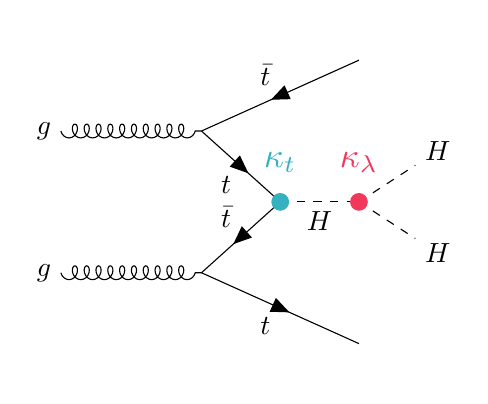
\begin{tikzpicture}
            \begin{feynman}
                \vertex (h1) at (0, 0);
                \vertex (h2) at (1, 0);
                \vertex (h3) at (2, 0.65) {\(H\)};
                \vertex (h4) at (2, -0.65) {\(H\)};

                \vertex(g1) at (-3, 0.9) {\(g\)};
                
                \vertex(t2) at (1, 1.8); %{\(t\)};
                \vertex(t1) at (-1, 0.9);
                
                \vertex(t3) at (-1, -0.9);
                \vertex(t4) at (1, -1.8); %{\(t\)};
    
                \vertex(g2) at (-3, -0.9) {\(g\)};
    
                \diagram*{
                    (g1) -- [gluon] (t1),
                    (t2) -- [fermion, edge label'=\(\bar{t}\)] (t1), 
                    (g2) -- [gluon] (t3),
                    (t3) -- [fermion, edge label'=\(t\)] (t4),
                    (t1) -- [fermion, edge label'=\(t\)] (h1),
                    (h1) -- [fermion, edge label'=\(\bar{t}\)] (t3),
                    (h1) -- [scalar, edge label'=\(H\)] (h2) -- [scalar] {(h3), (h4)},
                };
                    
            \end{feynman}
            
            \filldraw [hh_med_turq] (0, 0) circle (3pt);
            \node[hh_med_turq, scale=1.25] at (0, 0.5) {\(\kappa_{t}\)};
            
            \filldraw [hh_pink] (1, 0) circle (3pt);
            \node[hh_pink, scale=1.25] at (1, 0.5) {\(\kappa_{\lambda}\)};
            
            \filldraw [white] (0, 2.1) circle (3pt);
            \filldraw [white] (0, -2.1) circle (3pt);
            %PDF image cuts off just before bottom of diagram so put in a white dot to lower the lower edge.
            
        \end{tikzpicture}

\caption{Feynman Diagrams for the production of a resonance via Vector Boson Fusion and Gluon Gluon Fusion, which subsequently decays into a Higgs pair.}
\end{figure}

\end{document}
